\index{Preferences!Appearance}
\index{Appearance!Preferences}
\label{appearanceprefs}



\begin{figure}[h]
\begin{center}
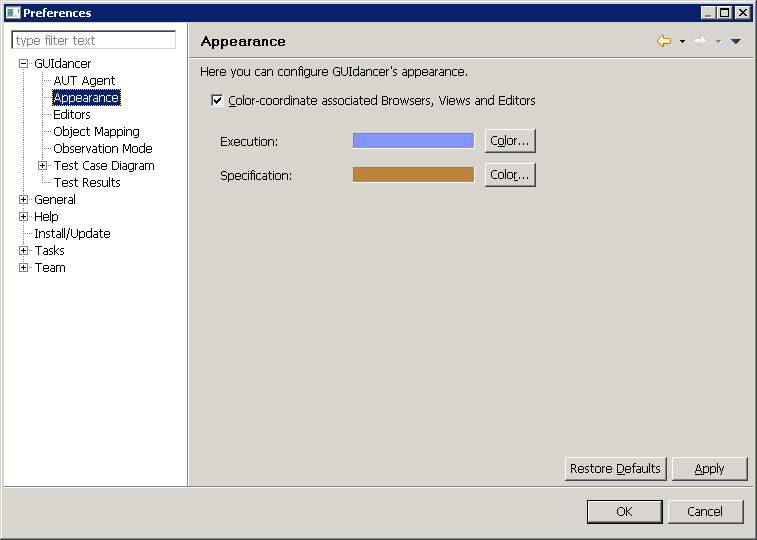
\includegraphics[width=12.5cm]{Tasks/Preferences/PS/appearanceprefs}
\caption{Appearance Preference Dialog}
\label{appearanceprefs}
\end{center}
\end{figure}

\begin{enumerate}
\item You can opt to color-coordinate browsers, editors and views which are related to each other. 
\item If you want to color-coordinate, you can choose your color scheme. 

\bxname{Execution} refers to the \gdtestsuitebrowser{}, the \gdtestsuiteeditor{} and the \gdpropview{}, \gdcompnamesview{} and \gddatasetsview{} for this editor. 

\bxname{Specification} refers to the \gdtestcasebrowser{}, the \gdtestcaseeditor{} and the \gdpropview{}, \gdcompnamesview{} and \gddatasetsview{} for this editor. 
\end{enumerate}






